\documentclass[12pt]{article}

\usepackage{graphicx}
\usepackage{amsmath}
\usepackage{geometry}
\geometry{a4paper, margin=1in}
\usepackage{hyperref}
\usepackage{booktabs}
\usepackage{pgfplots}
\pgfplotsset{compat=1.17}
\usepackage{float}

\begin{document}



\title{Predicting Cricket Match Outcomes Using Decision Trees and Random Forests}
\author{Parth Thakur\\
        2021CS50615}

\date{\today}

\section{Decision Trees and Random Forests}
\subsection{Decision Tree Construction}
    \begin{itemize}
        \item Constructed decision trees using mutual information for attribute selection.
        \item Handled continuous attributes through median-based splitting and categorical attributes through k-way splitting.
        \item Experimented with maximum depths of \{5, 10, 15, 20, 25\}.
    \end{itemize}


\begin{table}[H]
\centering
\caption{Decision Tree Accuracies at Various Depths}
\label{table:decision_tree_accuracies}
\begin{tabular}{ccc}
\toprule
Depth & Training Accuracy & Test Accuracy \\
\midrule
5  & 0.8855 & 0.5440 \\
10 & 0.9963 & 0.5657 \\
15 & 0.9969 & 0.5657 \\
20 & 0.9969 & 0.5657 \\
25 & 0.9969 & 0.5657 \\
\bottomrule
\end{tabular}
\end{table}

\begin{center}
    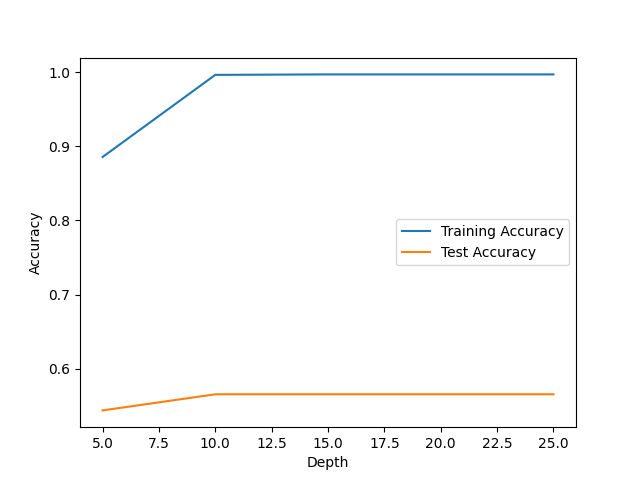
\includegraphics[width=0.8\textwidth]{Assignment 3/q1/(a)depth_vs_accuracy.png}
\end{center}

Training Accuracy for only loss prediction: 0.4966

Training Accuracy for only win prediction: 0.5033

Test Accuracy for only loss prediction: 0.5036

Test Accuracy for only win prediction: 0.4963

\begin{itemize}
    \item \textbf{Overfitting with Increasing Depth:} Training accuracy increases with depth, reaching nearly 99.7\% for depths 15, 20, and 25, indicating overfitting. Test accuracy remains constant around 56.57\% for depths above 10, suggesting the model doesn't generalize well to unseen data.
    
    \item \textbf{Consistent Test Accuracy:} Test accuracy is relatively consistent across different depths, suggesting that increased complexity at higher depths doesn't improve performance on unseen data.
    
    \item \textbf{Balanced Win/Loss Prediction:} Accuracies for only loss and only win prediction are roughly balanced around 50\%, indicating no significant bias towards predicting one class over the other.
    
    \item \textbf{Gap Between Training and Test Accuracies:} The significant gap between training and test accuracies, especially at higher depths, further indicates overfitting.
    
    \item \textbf{Optimal Maximum Depth:} A maximum depth of 10 appears to be a reasonable choice, offering a balance between training and test accuracies without excessive overfitting.
\end{itemize}


\subsection{Decision Tree One Hot Encoding}
    \begin{itemize}
        \item Implemented one hot encoding for categorical attributes.
        \item Repeated decision tree construction for depths \{15, 25, 35, 45\}.
        \item Compared results with the previous method.
    \end{itemize}

    \begin{table}[h]
\centering
\begin{tabular}{@{}ccc@{}}
\toprule
Max Depth & Training Accuracy & Test Accuracy \\ \midrule
15        & 0.7022            & 0.5574        \\
25        & 0.8398            & 0.6039        \\
35        & 0.9233            & 0.5926        \\
45        & 0.9868            & 0.6060        \\ \bottomrule
\end{tabular}
\caption{Accuracies of the decision tree with varying maximum depths.}
\end{table}

\subsection*{Observations}
\begin{itemize}
    \item The training accuracy increases with the depth of the tree, indicating a more complex model that better fits the training data.
    \item The test accuracy does not consistently improve with increased depth, suggesting that deeper trees may be overfitting the training data.
    \item The highest test accuracy is achieved at a depth of 45, but this comes with a significantly high training accuracy, which may imply overfitting.
    \item The depth of 25 offers a balance between training and test accuracies, potentially providing a model that generalizes better than deeper trees.
\end{itemize}

\subsection{Decision Tree Post Pruning}
    \begin{itemize}
        \item Applied post-pruning based on a validation set.
        \item Plotted training, validation, and test set accuracies against the number of nodes.
    \end{itemize}

\subsection{Decision Tree Sci-kit Learn}
    \begin{itemize}
        \item Built decision trees using the sci-kit learn library.
        \item Varying max depth in range \{15, 25, 35, 45\} and pruning parameters ccp alpha in range \{0.001, 0.01, 0.1, 0.2\}.
        \item Reported train and test accuracies and plotted against max depth and ccp alpha.
        \item Used validation set to determine optimal parameters.
        \item Compared results with parts (b) and (c).
    \end{itemize}

\subsection{Random Forests}
    \begin{itemize}
        \item Used sci-kit learn library to grow Random Forests.
        \item Experimented with parameters: n\_estimators (50 to 350), max\_features (0.1 to 1.0), min\_samples\_split (2 to 10).
        \item Performed grid search for parameter tuning based on out-of-bag accuracy.
        \item Reported training, out-of-bag, validation, and test set accuracies.
        \item Compared results with parts (c) and (d).
    \end{itemize}


\end{document}
